\documentclass{article}
\usepackage{tikz}

\usepackage[top=1cm, bottom=1cm, left=1cm, right=1cm]{geometry}

\begin{document}
\thispagestyle{empty}
\newcommand{\pos}{7}
\newcommand{\bod}{1.5}
\newcommand{\bodLen}{16}
\newcommand{\eh}{1}

% % % % % % % % % % % % % % % % % % % % % % % % % % % % % % % % % % % % % % % % % % % % % % % % % % % % % % % % % %
% first version, one color

\begin{figure}[!c]
	\centering
	\begin{tikzpicture}
	
	\fill[color=red] (-\pos,0) -- (0,\pos+\eh) -- (\pos,0)-- (-\pos,0);
	\fill[color=red] (-\bod,0) -- (\bod,0) -- (\bod,-\bodLen)-- (-\bod,-\bodLen);
	
	\end{tikzpicture}
\end{figure}


\clearpage
\thispagestyle{empty}
\begin{figure}[!c]
	\centering
	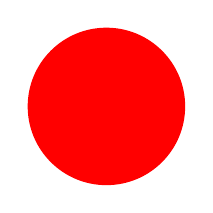
\begin{tikzpicture}
	\fill[color=red] (0,0) circle (\pos);
	\end{tikzpicture}
\end{figure}


\clearpage
\thispagestyle{empty}
\begin{figure}[!c]
	\centering
	\begin{tikzpicture}[rotate=45]
	\fill[color=red] (-\pos, -\bod)  -- (-\pos, \bod) -- (\pos, \bod)  -- (\pos, -\bod);
	\fill[color=red] (-\bod,-\pos)  -- (\bod,-\pos) -- (\bod,\pos)  -- (-\bod,\pos); 
	\end{tikzpicture}
\end{figure}


% % % % % % % % % % % % % % % % % % % % % % % % % % % % % % % % % % % % % % % % % % % % % % % % % % % % % % % % % %
% second version, with blue boundaries around
\clearpage
\pagestyle{empty}

\begin{figure}[!c]
	\centering
	\begin{tikzpicture}[scale=0.9]
	\begin{scope}
		\fill[color=blue] (-\pos-2*\eh,-\eh) -- (0, 2.41*\eh+\pos) -- (2*\eh+\pos, -\eh);
		\fill[color=blue] (-\eh-\bod,0) -- (\eh+\bod,0) -- (\eh+\bod, -\eh-\bodLen)-- (-\eh-\bod,-\eh-\bodLen);
	\end{scope}
	
	\fill[color=red] (-\pos,0) -- (0,\pos+\eh) -- (\pos,0)-- (-\pos,0);
	\fill[color=red] (-\bod,0) -- (\bod,0) -- (\bod,-\bodLen)-- (-\bod,-\bodLen);
	

	\end{tikzpicture}
\end{figure}


\clearpage
\thispagestyle{empty}
\begin{figure}[!c]
	\centering
	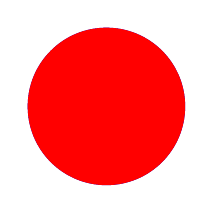
\begin{tikzpicture}
	\fill[color=blue] (0,0) circle (\pos+\eh);
	\fill[color=red] (0,0) circle (\pos);
	\end{tikzpicture}
\end{figure}


\clearpage
\thispagestyle{empty}
\begin{figure}[!c]
	\centering
	\begin{tikzpicture}[rotate=45]
		\fill[color=blue] (-\pos-\eh, -\eh-\bod)  -- (-\eh-\pos, \eh+\bod) -- (\eh+\pos, \eh+\bod)  -- (\eh+\pos, -\eh-\bod);
		\fill[color=blue] (-\eh-\bod,-\eh-\pos)  -- (\eh+\bod,-\eh-\pos) -- (\eh+\bod,\eh+\pos)  -- (-\eh-\bod,\eh+\pos); 
		
	\fill[color=red] (-\pos, -\bod)  -- (-\pos, \bod) -- (\pos, \bod)  -- (\pos, -\bod);
	\fill[color=red] (-\bod,-\pos)  -- (\bod,-\pos) -- (\bod,\pos)  -- (-\bod,\pos); 

	\end{tikzpicture}
\end{figure}



\end{document}